\documentclass[12pt,convert={false}]{standalone}
\usepackage[dvipsnames]{xcolor}
\usepackage{tikz}
\usetikzlibrary{shapes,arrows,positioning,calc,patterns,arrows.meta, bending, graphs, shadings,quotes,intersections}
\usetikzlibrary{external}
%\tikzexternalize[prefix=tikz/]
\usepackage{pgfplots}
\pgfplotsset{compat=1.16}
\usepgfplotslibrary{fillbetween}
\newcommand{\enf}[1]{\textcolor{RedViolet}{\textbf{#1}}} %enf sta per enfasi
\newcommand{\sott}[1]{\setulcolor{black!20!Goldenrod}\ul{#1}}
\newcommand{\prob}{\mathbb{P}}
\newcommand\independent{\protect\mathpalette{\protect\independenT}{\perp}}
\newcommand{\ev}[1]{\mathbb{E}\Bigl[{#1}\Bigr]}
\def\independenT#1#2{\mathrel{\rlap{$#1#2$}\mkern2mu{#1#2}}}
\newcommand{\Z}{\mathbb{Z}}
\newcommand{\R}{\mathbb{R}}
\newcommand{\N}{\mathbb{N}}
\newcommand{\equalexpl}[1]{%
	\underset{\substack{\uparrow\\\mathrlap{\text{\vspace{-3cm}\hspace{-1em}#1}}}}{=}}
\newcommand{\dif}{\mathop{}\!\mathrm{d}}
\begin{document}
 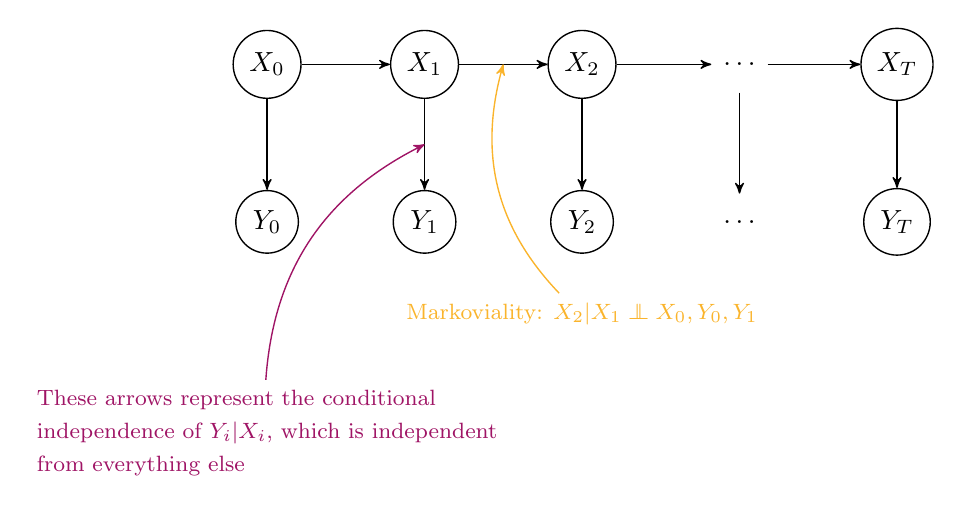
\begin{tikzpicture}[->,>=stealth', line width=0.5pt, node distance=2cm]
	\node [circle,draw] (x0) [] {$X_0$};
	\node [circle,draw] (x1) [right of= x0] {$X_1$};
	\node [circle,draw] (x2) [right of= x1] {$X_2$};
	\node [circle] (dots) [right of= x2] {$\ldots$};
	\node [circle,draw] (xt) [right of= dots] {$X_T$};
	\node [circle,draw] (y0) [below of=x0] {$Y_0$};
	\node [circle,draw] (y1) [right of= y0] {$Y_1$};
	\node [circle,draw] (y2) [right of= y1] {$Y_2$};
	\node [circle] (ydots) [right of= y2] {$\ldots$};
	\node [circle,draw] (yt) [right of= ydots] {$Y_T$};
	\node [align=left] (indep) [RedViolet,below=1.6cm of y0] {\footnotesize These arrows represent the conditional \\ \footnotesize independence of $Y_i|X_i$, which is independent\\ \footnotesize from everything else};
	\node [align=left] (markoviality) [Dandelion,below=0.5cm of y2] {\footnotesize Markoviality: $X_2|X_1\independent X_0,Y_0, Y_1$};
	\path (x0) edge (x1);
	\draw[->] (x1) -- (x2) node [sloped,midway](L){};
	\path (x2) edge (dots);
	\path (dots) edge (xt);
	\path (x0) edge (y0);
	\draw[->] (x1) -- (y1) node [sloped,midway](M){};
	\path (x2) edge (y2);
	\path (dots) edge (ydots);
	\path (xt) edge (yt);
	\draw[->,RedViolet] (indep) to[bend left] (M.center);
	\draw[->,Dandelion] (markoviality) to[bend left] (L.center);
\end{tikzpicture}
\end{document}
